\chapter{Structure of the Game}
The structure of the grid-based strategy war game is designed to provide a seamless and engaging experience while integrating dynamic interactions with an LLM-driven NPC enemy commander. 
\section{Grid Based Map}
The battlefield is represented as a grid-based map, where both the player and the enemy commander can deploy their units on valid areas. \ref{fig:Grid-Based-Map}.
\begin{figure}[!htbp]
    \centering
    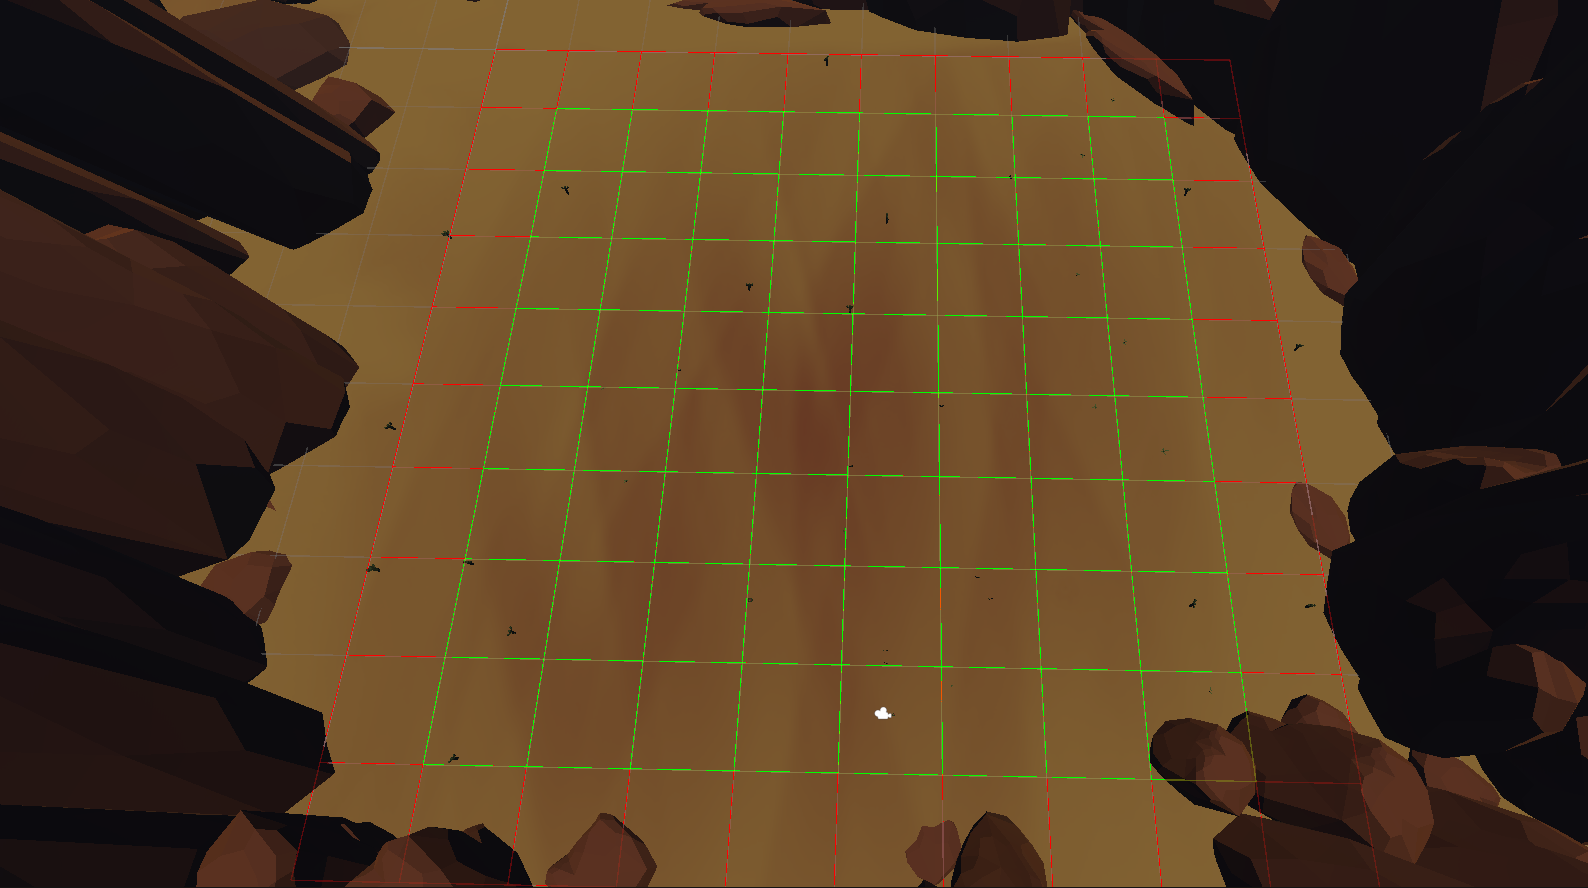
\includegraphics[width=0.5\linewidth]{map_grids.png}
    \caption{Grid Based Map}
    \label{fig:Grid-Based-Map}
\end{figure}

\section{Player Mechanics}
The player assumes the role of a commander with the ability to interact with the game world and the enemy commander.

\begin{itemize}
    \item The player can place soldiers, tanks, and throw airstrikes onto the map.
    \item The player can engage in dialogue with the enemy commander to negotiate surrender or to provoke them.
\end{itemize}

\section{Enemy Commander}
The enemy commander is powered by a large language model (LLM) and plays a pivotal role in the game.
\begin{itemize}
    \item The enemy commander interacts with the player through contextual dialogue, responding to game state changes and player actions.
    \item The NPC adjusts its "aggressiveness" and "surrender likelihood" values based on the evolving game state. (If player provokes NPC, aggressiveness increase and if the battle is going against NPC, surrender likelihood increase.)
    \item The NPC exhibits more aggressive dialogue when its aggressiveness value is high.
\end{itemize}

\section{Unit Types}
The game features three primary unit types, each with distinct roles and abilities:
\begin{itemize}
    \item \textbf{Soldiers}: Infantry units equipped with rifles that deal direct damage to targeted enemies.
    \item \textbf{Tanks}: Tank units capable of delivering area damage around a targeted enemy.
    \item \textbf{Airstrikes}: Aerial projectiles that inflict area damage at a specified location, offering strategic advantages in eliminating clusters of enemies.
\end{itemize}

\section{Victory Conditions}
The game ends when one of the following conditions is met:
\begin{itemize}
    \item \textbf{Player Victory}: Achieved by either forcing the enemy commander to surrender or eliminating all enemy units.

    \item \textbf{Enemy Victory}: The player loses if their units are obliterated.
\end{itemize}

\section{Level Design Window}
The level design window enables players to customize game settings, providing flexibility and variety for gameplay scenarios.

\subsection{Interface Overview}
The interface includes:
\begin{itemize}
    \item \textbf{Unit Configuration}: Input fields for setting player and enemy soldiers, tanks, and airstrikes.
    \item \textbf{Aggressiveness Slider}: Adjusts the enemy's behavior dynamically.
    \item \textbf{Language Button}: Toggles between English and Turkish for NPC dialogue.
    \item \textbf{Start Button}: Launches the game with the selected settings.
\end{itemize}

\subsection{Impact on Gameplay}
The level design window allows players to:
\begin{itemize}
    \item Customize difficulty by modifying unit counts and aggressiveness.
    \item Tailor gameplay scenarios to test strategies and configurations.
\end{itemize}

\subsection{Example Configuration}
A sample setup could include 30 soldiers, 10 tanks, and 5 airstrikes for the player; 40 soldiers, 8 tanks, and 7 airstrikes for the enemy; and an aggressiveness value of 3. \ref{fig:level-design-window}
\begin{figure}[!htbp]
    \centering
    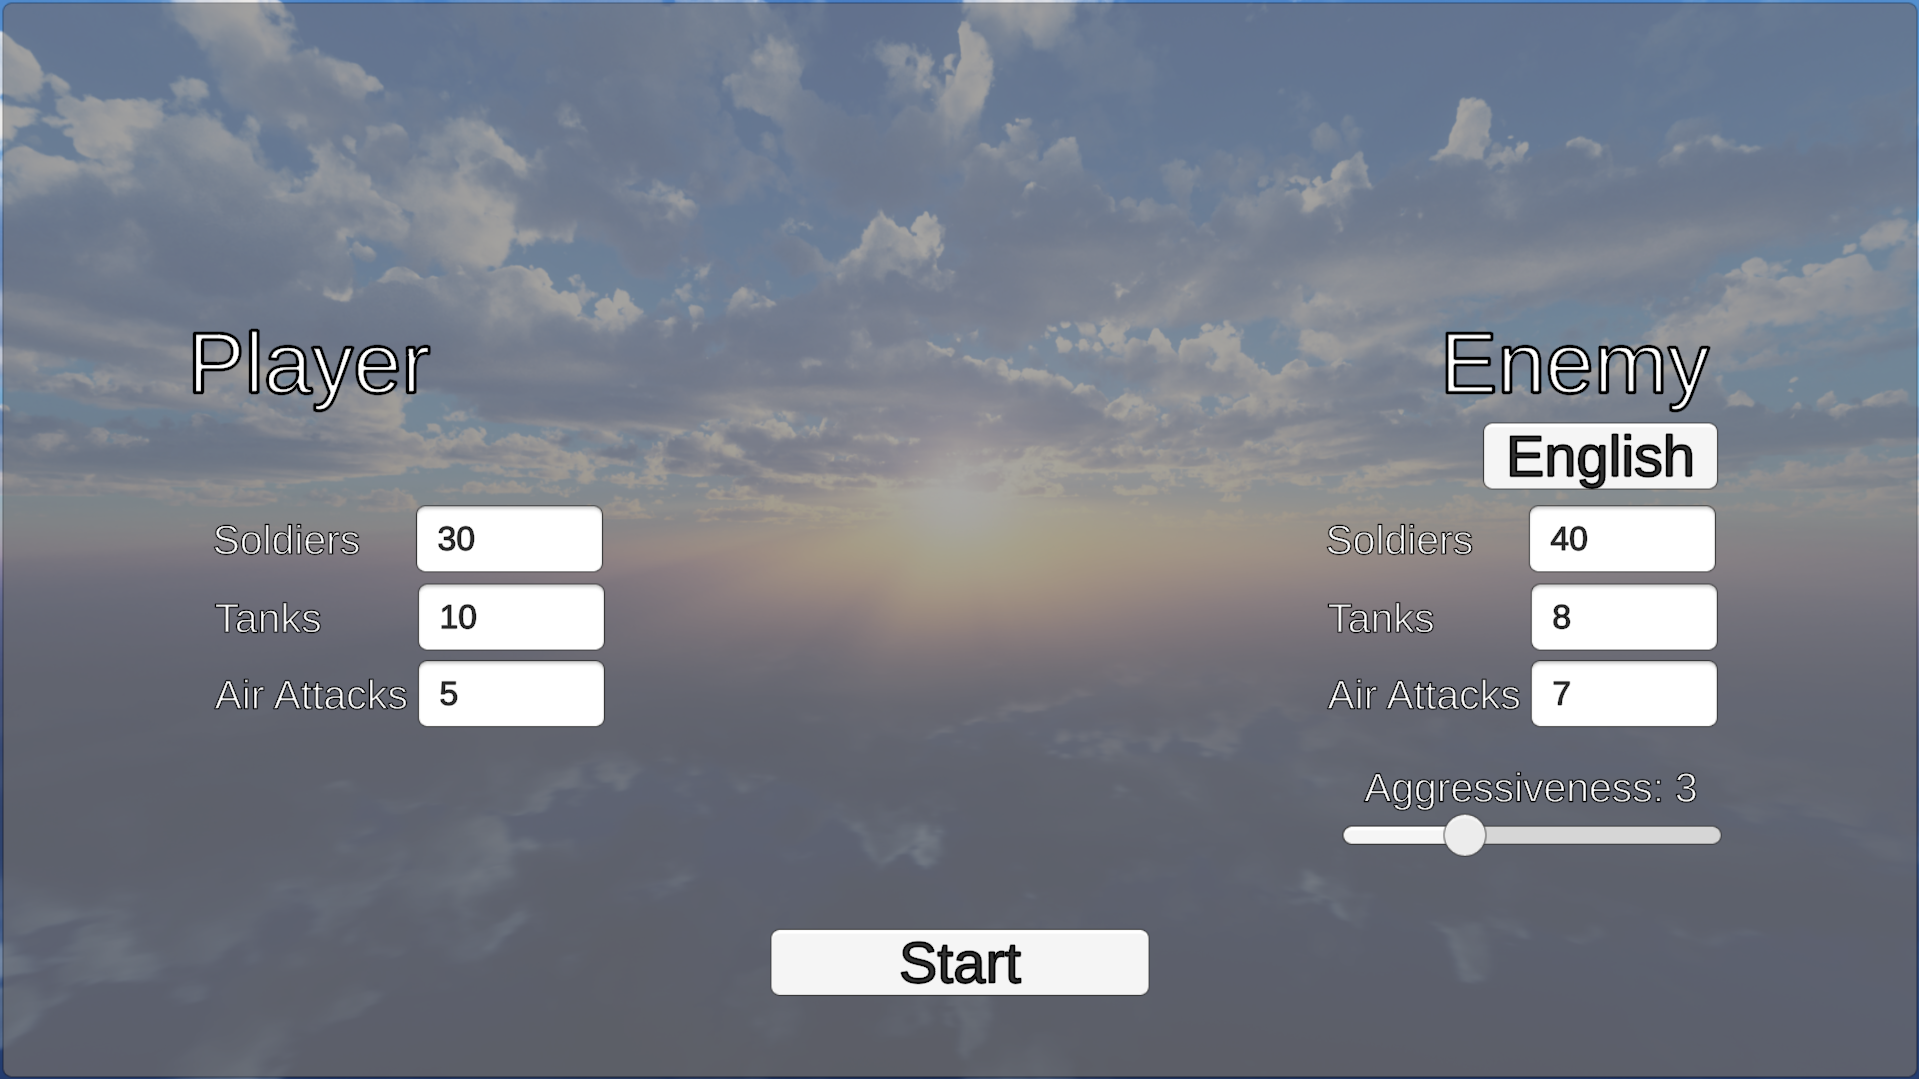
\includegraphics[width=1.0\linewidth]{image.png}
    \caption{Level Design Window}
    \label{fig:level-design-window}
\end{figure}





